\chapter{Implementació}
\label{sec:implementacio}

En aquest capítol es descriuen les parts més importants de l'implementació del projecte tot justificant les decisions preses i descrivint totes les alternatives estudiades. 

La secció \ref{sec:implementacio-overall} dóna una visió general de l'estructura de l'implementació de l'algorisme. Les següents seccions expliquen cadascun dels mòduls esmentats a la visió general. Finalment, s'inclou la secció \ref{sec:implementacio-llenguatge} on es justifica l'elecció de llenguatge de programació per a aquest projecte.

\section{Estructura general de l'algorisme}
\label{sec:implementacio-overall}

L'algorisme per comparar descripcions textuals i models BPMN s'ha implementat seguint una estructura similar a la formalització proposada a l'apartat \ref{cha:enfoc}. A la figura \ref{fig:implementacio-diagram} es pot veure l'estructura de mòduls que conformen l'algorisme.

Per consultar el codi font del programa, veure l'annex \ref{cha:codi_font}.

\begin{figure}[!h]
    \includegraphics[width=\textwidth]{diagrams/Implementacio_Diagrama.png}
    \caption{Estructura general de l'implementació de l'algorisme.}
    \label{fig:implementacio-diagram}
\end{figure}

\section{Preprocessat de les dades d'entrada}
\label{sec:implementacio-preprocessat}

El primer pas que realitza l'algorisme és un pre-tractament de les dades d'entrada perquè es puguin analitzar fàcilment a les següents fases d'aquest. En aquesta secció es descriu el preprocessat que segueixen les dades d'entrada de l'algorisme: El text pla en llenguatge natural i el model BPMN.

\subsection{El text analitzat}
\label{sec:implementacio-preprocessat-text}

Pel que fa a l'anàlisi del text, l'objectiu és obtenir una estructura de dades que reflexi l'estructura sintàctica del text a partir del text pla d'entrada.

Aquesta tasca no s'ha implementat en aquest projecte, sinó que s'usa la llibreria \emph{Freeling} per al processat del text en llenguatge natural, deixant per a aquest projecte la tasca d'interpretar aquesta informació. \emph{Freeling} tampoc s'ha integrat com una llibreria en el projecte, sinó que s'utilitza la API http del \emph{Textserver}. La decisió d'utilitzar el \emph{Textserver} en comptes de \emph{Freeling} com una llibreria nativa ve motivada per dues raons. La primera és el pes de la llibreria, ja que requereix els diccionaris de Wordnet en diversos idiomes. D'altra banda \emph{Freeling} està programat en C++, cosa que implica que caldria incloure'l compilat per a diversos sistemes operatius i arquitectures si es volgués una solució portable en Java. La segona raó és la simplicitat de programació. Tot i que \emph{Freeling} ofereix una interfície nativa per a java (JNI), resulta més senzill navegar una única estructura de dades en un format estàndard com JSON.

Per l'anàlisi del text es crida al mètode \emph{semgraph} del \emph{Textserver} que realitza una anàlisi més complet del text. L'anàlisi que realitza el \emph{Textserver} conté, entre altres coses:

\begin{itemize}
    \item El text separat en frases i l'anàlisi morfològic de cadascuna de les paraules.
    \item La llista de predicats\footnote{No només els predicats verbals, sinó totes aquelles parts de la frase que impliquin alguna acció, es consideren predicats en aquest cas.} que conté cadascuna de les frases.
    \item L'arbre de constituents de les frases.
    \item L'arbre de depencències de les frases.
    \item El graf semàntic del text.
\end{itemize}

\subsection{El model BPMN}
\label{sec:implementacio-preprocessat-model}

Pel que fa al model BPMN, s'han considerat dues parts diferenciades. Per una banda, el BPMN conté tota l'estructura formal, en forma de dades estructurades. D'altra banda, els diferents elements del BPMN, també contenen text en llenguatge natural. És per això que s'han plantejat dos preprocessats diferents per al BPMN.

El primer preprocessat consisteix simplement a obtenir l'informació estructural del BPMN i representar-la en un format adient. Per a fer la lectura del model, s'usa el parser de la llibreria Activiti, que ja implementa la lectura dels models BPMN. No obstant això, Activiti no és una llibreria pensada per llegir BPMNs, sinó per executar-los. És per això que les funcionalitats que exposa estan enfocades a un altre tipus de programes. L'alternativa a Activiti hagués estat implementar la lectura dels models BPMN, tot i això, s'ha desestimat per evitar els possibles contratemps que els errors en un parser propi poguéssin introduir.

El segon preprocessat correspon a analitzar el text, en llenguatge natural, contingut al model. Per a fer-ho, s'usa novament la llibreria \emph{Freeling}. Tot i això, alguns dels processats que realitza la llibreria, com la detecció de senses requereixen d'un cert context. Per exemple, en català, la paraula ``gat'' se sol referir típicament a l'animal, però si en el text apareixen paraules com ``taller'', ``cotxe'' i ``reparació'', freeling farà servir aquesta informació de context per determinar que no es tracta pas de l'animal, sinó de l'eina. Com que les frases del model BPMN típicament són senzilles, i per tant no contenen prou context, s'afegeixen les frases del text a l'anàlisi. Així, si el vocabulari del text i el model estan en un àmbit similar, la detecció del significat de cada paraula es realitzarà correctament. Finalment, les frases del text original es descarten i queda el text del model analitzat. 

\section{Extracció de característiques}
\label{sec:implementacio-extraccio}

Un cop l'informació d'entrada ha estat degudament preprocessada, el següent pas que realitza l'algorisme és l'extracció de característiques. Una vegada més, la tasca s'ha dividit en dos mòduls separats per al text i el model, ja que la seva representació no és uniforme. 

En el mòdul d'extracció de característiques es declaren quines són les característiques que s'extrauran del text i del model. Cada característica es defineix amb un pes, això permet donar més importància a que el text i el model comparteixin subjecte que no pas que comparteixin una paraula. Aquest pes s'utilitza després en el càlcul de similaritat i està determinat manualment.


Aquest és el conjunt de característiques que s'han considerat a l'hora d'implementar l'algorisme\footnote{Els noms que es fan servir són els mateixos que en el codi, per facilitar la comprensió d'aquest.}. Seguint el formalisme descrit a l'apartat \ref{sec:enfoc-extraccio}, es descriu cada tipus de característica amb el nom i arguments.

\begin{description}
    \item[Has-Lemma(pos, lemma): ]{El text conté una paraula amb arrel \textbf{lemma} i categoria gramatical \textbf{pos}.}
    \item[Has-action(a):]{El text descriu una acció representada per la paraula \textbf{a}, generalment un verb.}
    \item[Has-Synset(s):]{El text conté una paraula que pertany al synset \textbf{s} al diccionari de Wordnet 3.0\footnote{La versió del diccionari pot canviar, però és la que utilitza Freeling i per tant la que s'utilitza en aquest projecte.}}
    \item[Has-Parent-Synset(s):]{El text una paraula el synset de la qual és un homònim del synset \textbf{s}. És a dir, la paraula i \textbf{s} tenen una relació de \emph{és un}.}
    \item[In-Agent(lemma, pos, verb):]{El rol d'agent de l'acció \textbf{verb} conté la paraula amb arrel \textbf{lemma} de categoria gramatical \textbf{pos}}
    \item[In-Patient(lemma, pos, verb):]{El rol de pacient de l'acció \textbf{verb} conté la paraula amb arrel \textbf{lemma} de categoria gramatical \textbf{pos}}
    \item[Lemma-conditional-pred(lemma, pos)]{El text, o tasca, segueix una condició que conté la paraula \textbf{lemma} de categoria gramatical \textbf{pos}.}
\end{description}

El més important d'aquestes característiques és que han de ser rellevants tant pel text com pel model. Es podria extreure informació molt més complexa de cadascun dels dos per separat, però no existiria una versió homòloga a l'altre. 

És important notar també que moltes vegades s'inclou informació addicional com la categoria gramatical o el verb, en el cas d'agents i pacients. Això es fa per concretar les característiques. Per exemple, si dos fragments de text contenen la paraula ``document'' --en anglès-- però en una apareix com a verb i l'altre com a nom, no haurien de contribuir a la similaritat total.

La característica \textbf{Has-Parent-Synset} s'utilitza per detectar paraules que no són sinònims directes. Per exemple, es pot donar el cas que el text parli d'un ``document'' que s'ha dit que és una carta, però al model s'utilitzi sempre la paraula ``carta''. Quan el model parli de carta i el text de document, ni les paraules ni els synsets coincidiràn\footnote{Carta i document no són sinònims en general, tot i que puguin ser-ho en el text.} però si que ho farà algun dels seus hiperònims. No obstant això, per evitar crear falsos positius amb aquestes característiques, cada cop que es va amunt en la cadena d'hiperonimia, el pes de la característica es multiplica per un cert valor fent que vagi disminuint.

La característica \textbf{In-Agent} serveix per identificar el rols semàntics d'agent en una frase o tasca. L'agent d'una acció respon a la pregunta ``Qui?'', és a dir, indica qui realitza l'acció. L'extracció d'aquesta característica és molt diferent entre el text i el model. En una frase, identificar l'agent és una tasca purament de processat de llenguatge natural i s'ha implementat utilitzant Freeling. D'altra banda, per identificar l'agent d'una tasca en el model, es fa servir la semàntica del BPMN. En un model BPMN l'agent que realitza cadascuna de les accions s'ha d'explicitar mitjançant les \emph{pools} i les \emph{swimlanes}, així que l'informació s'obté directament del model.

Finalment, per cadascuna de les característiques declarades, s'implementa una funció extractora pel text i pel model. És a dir, una funció que, rebent el text analitzat en retorna un vector de característiques i anàlogament pel model. És important notar que el text i el model són estructures totalment diferents, i que l'objectiu d'aquest mòdul és crear una representació comú. Així doncs, és necessari tenir per duplicat cadascuna de les funcions extractores, pel text i pel model, ja que el codi de cadascuna d'aquestes pot des de tenir lleugeres diferències fins a ser conceptualment diferent. El resultat d'aquestes funcions extractores correspon al resultat del mòdul d'extracció.

\section{Càlcul de la similaritat}
\label{sec:implementacio-similaritat}

Establir una noció de similaritat entre frases del text i taques del model és complicat. No obstant, un cop redüit el problema a vectors de característiques, existeixen tot tipus de mètriques a la literatura. En concret, l'implementació d'aquest mòdul ha consistit a implementar les diferents mètriques de similaritat descrites a l'apartat \ref{sec:enfoc-similaritat}. L'implementació és una traducció directa de les fórmules.

Aquest mòdul també permet escollir, mitjançant una opció de configuració, quina és la mètrica de similaritat que es vol exposar.

Com a valor per defecte s'ha escollit utilitzar l'índex d'Overlapping ponderat. Degut a la naturalesa del problema amb el que es tracta, les frases del text sempre solen ser més verboses que les frases del model i, per tant, contenen més paraules. Això fa que el conjunt de features de les frases del text sigui quasi sempre més gran que el de les frases del model. En les altres funcions de similaritat, aquesta diferència de cardinalitat fa que el valor, tot i ser correcte a nivell relatiu, acabi tenint un valor molt baix en magnitud. L'índex d'Overlapping té la propietat que dos conjunts tenen una similaritat màxima de $1$ si el petit és subconjunt del gran. Per aquest fet, l'índex d'Overlapping, i la seva versió ponderada, dónen resultats numèrics molt més intuitius\footnote{Utilitzant cosinus o jaccard ponderat, la similaritat d'una parella de model-text bona és de l'ordre de $0.1$, mentre que si la parella és dolenta el valor de l'ordre de $0.001$. Utilitzant l'índex d'Overlapping aquests valors passen a ser $0.5$ i $0.01$.} de cara a mostrar una puntuació a l'usuari final. No obstant això, l'objectiu no és sempre donar una puntuació intuitiva. És possible que a l'hora de comparar, els resultats obtinguts d'altres mètriques de similaritats siguin més precisos a nivell relatiu.

El resultat d'auqest mòdul és, finalment, la matriu de similaritat. La matriu de similaritat és una matriu $|S|\times|T|$ l'element $(i,j)$ de la qual indica la similaritat entre la frase $i$ i la tasca $j$.

\section{Ordenació de models i textos}
\label{sec:implementacio-ordenacio}

El mòdul d'ordenació s'estructura, novament, en dues parts. L'ordenació de textos i de models. L'ordenació de textos, tal com s'explica a l'apartat \ref{sec:enfoc-ordre-text}, és una gran simplificació respecte el problema real. Així doncs, en aquest apartat només es parla de l'ordenació de tasques al model.

El resultat del mòdul son dues matrius, una pel text i una pel model. En aquestes dues matrius, cada element pot prendre els valors: $\rightsquigarrow$, $\leftsquigarrow$ i $\neq$. Els dos primers valors representen les relacions ``Precedeix a'' i ``Succeeix a''. Així doncs, la matriu indica per cada cada element $(i,j)$ la relació d'ordre entre l'element $i$ i el $j$\footnote{A la matriu del text $i$ i $j$ son frases, a la del text tasques.}. 

\subsection{Al model}
\label{sec:implementacio-ordenacio-model}

Com s'explica a la secció \ref{sec:enfoc-model} l'ordenació de tasques al model es fa mitjançant el càlcul del \emph{Behavioral Profile}\cite{behavioral_profiles} del model. Cal notar que si s'intentés implementar el càlcul a partir de la definició formal, el cost d'aquest algorisme seria exponencial, havent de tractar tots els possibles camins del graf de procés. No obstant, existeixen algorismes molt més eficients a la literatura. Com que l'implementació d'auqests algorismes és bastant complexa, s'ha usat la llibreria JBPT (Business Process Technologies for Java) que implementa el càlcul dels behavioral profiles. També s'ha implementat l'algorisme de postprocessat, aquest s'ha implementat tal com es defineix a la secció \ref{sec:enfoc-ordre-model}.

Tot i això, els \emph{Behavioral Profiles} no van ser la primera alternativa estudiada. Primer de tot, es va plantejar aquest problema com una ordenació topològica del graf de processos. Com que els grafs de processos no son acíclics, per a plantejar aquest enfoc és necessari un algorisme d'eliminació de \emph{back-edges} considerant el BPMN un graf de flux\cite{dragon_book}. Aquest procediment està implementat al projecte, però es va descartar ja que els resultats que donava no eren exactament el tipus d'ordre que es volia modelar.

\section{Càlcul de la correspondència òptima}
\label{sec:implementacio-correspondencia}

L'objectiu d'aquest mòdul és calcular una aplicació de tasques a frases que satisfaci les tres restriccions definides a l'apartat \ref{sec:enfoc-matching}: Assignació total, Optimalitat i Consistència d'Ordre. La primera és una propietat inherent al problema. La segona fa referència a la matriu de similaritats. La tercera es pot veure com un conjunt de restriccions en funció de la matriu d'ordre. 

Per implementar aquest apartat s'han plantejat diverses alternatives. L'opció escollida finalment ha estat el modelar el problema com un programa ILP (Integer Linear Programming). No obstant això les tres solucions estudiades tenen els seus punts forts i febles. Com es pot veure a la figura \ref{fig:comparativa-algorismes}, LAP destaca per ser el més eficient dels tres algorismes, tot i trobar solucions de menor qualitat. D'altra banda, la qualitat de les solucions amb CP i ILP és la mateixa. No obstant això, donada la major flexibilitat que ofereix Constraint Programming, aquest es planteja com a solució alternativa en cas que noves restriccions introduides al problema en un futur féssin que ILP deixés de ser una alternativa viable.

\begin{figure}[htb]
    \centering
    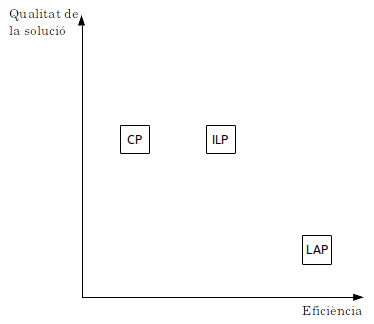
\includegraphics[width=0.6\textwidth]{figures/algorithm_comparison.png}
    \caption{Comparativa dels diferents algorismes estudiats.}
    \label{fig:comparativa-algorismes}
\end{figure}

En els següents apartats es descriu en més detall cadascuna de les diferents alternatives plantejades i es justifica l'elecció de ILP com a millor opció per a resoldre el problema.

\subsection{Reducció a LAP}
\label{sec:implementacio-lap}

El LAP (Linear Assignment Problem)\cite{LAP} es pot formular, informalment, de la següent manera:
\begin{displayquote}
    Una instància del problema correspon a un conjunt $A$ de $N$ d'\emph{agents} i un conjunt de $T$ de $N$ \emph{tasques}. Per cada agent es disposa del cost que suposa assignar-lo a una tasca concreta. L'objectiu és trobar l'assignació que assigna cada agent a una tasca diferent minimitzant el cost total.
\end{displayquote}

Com es pot veure, aquest problema guarda una certa relació amb el que s'ha de resoldre en aquest cas. Tots dos problemes busquen trobar una assignació entre elements de dos conjunts tot minimitzant una funció objectiu. Tot i això, un LAP no contempla cap mena de consistència d'ordre.

La solució proposada és adaptar les condicions del problema original per aconseguir una instància d'un LAP. Per fer-ho, calen dues coses: Codificar l'ordre i aconseguir el mateix nombre de tasques i frases. Per codificar l'ordre, cal canviar el concepte d'ordre pel de distància, multiplicant la similaritat entre cada tasca i frase, per la inversa de la distància entre aquests. La intuició darrere ponderar per la distància inversa és penalitzar solucions on, per exemple, s'assignen dues frases consecutives a dues tasques molt separades en el mdodel; creant una noció d'ordre similar a la de la restricció original. Pel que fa a tenir el mateix nombre de tasques i frases, es pot resoldre ampliant el conjunt més petit amb elements falsos amb similaritat 0 per qualsevol altre element. Així, l'algorisme assignarà els pitjors candidats del matching a aquests elements falsos.

La motivació darrere aquesta idea és que LAP té solució en temps polinòmic, cosa que faria que tot l'algorisme es pogués executar en temps polinòmic. Si la relaxació de les condicions resulta ser massa forta, el resultat del LAP es podria seguir utilitzant com a solució inicial per algun algorisme d'optimització global.

Tot i això, un cop portada a la pràctica, aquesta solució no va donar els resultats esperats. El problema és que el resultat del LAP ha de ser una assignació bijectiva. Mentre que la naturalesa d'aquest problema fa que, moltes vegades, l'assignació òptima sigui justament no bijectiva. Per exemple, poden existir frases en el text que serveixin d'introducció per al lector i que no es refereixin a cap acció concreta. D'altra banda, també és comú el cas que una frase correspongui a dues tasques (una conjunció de dues accions, per exemple). Aquestes diferències entre la natrualesa dels problemes han fet que es descartés aquesta opció.

\subsection{Constraint Programming}
\label{sec:implementacio-cp}

La segona alternativa plantejada consisteix a modelar el problema com un conjunt de restriccions per a un solver de constraint programming\cite{CP}. Una bona alternativa per a aquestes tasques és Choco Solver, una llibreria de sofware lliure per a Java que permet modelar problemes de satisfacció de restriccions.

Per modelar el problema com un CSP s'han estudiat dues alternatives.

La primera alternativa defineix el conjunt de variables $T$ com el conjunt de tasques, cadascuna amb el domini de valors $1 \cdots |S|$, on $|S|$ és el nombre total de tasques. Es considera que la frase $i$ i la tasca $j$ estan relacionades si $T_j = i$. A més, s'afegeixen les variables auxiliars $Sim_1 \cdots Sim_{|T|}$, on $|T|$ és el nombre de frases. A les variables se'ls hi imposen les restriccions següents: 
\begin{itemize}
    \item Per cada tasca $T_i$: $T_i = j \implies Sim_i = SM_{ij}$, on $SM$ és la matriu de similaritats.
    \item Per cada parella de tasques $T_i$, $T_j$ una restricció: $TO_{ij} = \rightsquigarrow \implies T_i <= T_j$, on $TO$ és la matriu d'ordre del model. 
    \item A més, s'indica al solver que maximitzi l'expressió: $\sum_i^{|S|}{Sim_i}$.
\end{itemize}

És fàcil veure que aquesta codificació compleix amb totes les restriccions imposades. La optimalitat la garantitza el solver maximitzant la suma de les similaritats, mentre que la consistència d'ordre la garanteix la segona restricció. D'aquesta segona restricció, cal notar que es fa servir el truc que les frases tenen un ordre seqüencial per considerar l'ordre entre frases igual a l'ordre dels enters que les representen.

La segona alternativa fa servir variables booleanes $A_{ij}$ = ``La tasca $i$ s'ha assignat a la frase $j$''. En aquesta nova codificació, les restriccions són:

\begin{itemize}
    \item Per cada valor $i$: $\sum_j{A_{ij}} = 1$.
    \item Per cada parella $(s, s')$ de frases i cada parella $(t, t')$ de tasques: ($TO_{tt'} = \rightsquigarrow$ i $SO_{ss'} = \leftsquigarrow$ $\implies$ $\lnot (A_{s,t} \land A_{s',t'})$, on $TO$ i $SO$ son les matrius d'ordre del model i el text respectivament.
    \item A més, s'indica al solver maximitzar l'expressió $\sum_i^{|S|}{\sum_j^{|T|}{A_{ij} * SM_{ij}}}$
\end{itemize}

Les dues alternatives donen un resultat equivalent, i compleixen amb les restriccions del problema. No obstant això, el temps d'execució d'algunes instàncies del problema amb Choco Solver són massa elevats, arribant a trigar fins a 7 minuts. La diferència de temps entre les dues alternatives no és significativa. Aquest temps d'execució és massa gran pel tipus de software que es vol desenvolupar, per això es va descartar Constraint Programming com alternativa en general. Tot i això, si les restriccions del problema fóssin més complexes seria interessant tornar a estudiar aquesta alternativa, ja que Constraint Programming és un enfoc totalment genèric a resoldre problemes de restriccions que permet una màxima flexibilitat i és molt senzill d'utilitzar.

\subsection{Integer Linear Programming}
\label{sec:implementacio-ilp}

Un subconjunt dels problemes de satisfacció de restriccions és la programació entera. Un programa per a un solver de ILP\cite{ILP}, o \emph{linear program}, és un conjunt d'inequacions lineals definides sobre un conjunt de variables enteres\footnote{O booleanes, com a cas especial dels enters amb domini $\{0,1\}$}.

Partint de la segona formulació plantejada en el mètode de Constraint Programming, un conjunt de variables booleanes $A_{ij}$, es poden redefinir les restriccions del problema anterior com inequacions lineals\footnote{Afegint variables auxiliars addicionals, els solvers de ILP també permeten modelar equacions, aquest pas el realitza automàticament el solver.}. Fixant-nos en les tres restriccions de l'apartat anterior, la 1 i la 3 ja són equacions enteres, així doncs no cal fer res. Pel que fa a la segona restricció, l'expressió booleana $\lnot (A_{s,t} \land A_{s',t'})$ es pot reinterpretar com: $A_{s,t} + A_{s',t'} \leq 1$. Aquesta transformació permet adaptar la formulació de l'apartat anterior a un \emph{linear program}.

Aquesta codificació del problema és equivalent a les de l'apartat anterior, i per tant compleix les restriccions imposades. D'altra banda utilitzant un solver senzill de ILP (\emph{lp\_solve}), els temps d'execució pels problemes difícils es redueixen de minuts a milisegons, cumplint perfectament les expectatives del software que es vol obtenir. Aquesta reducció tant dràstica de temps es dóna ja que el solver de ILP és capaç d'assumir més coses sobre l'espai de cerca, ja que el problema es planteja de manera molt més concreta que no pas amb Constraint Programming.

\section{Mostra dels resultats}
\label{sec:implementacio-resultats}

La funció d'aquest últim mòdul és recopilar tota l'informació obtinguda per a mostrar-la a l'usuari. Com més informació es mostri del funcionament intern de l'algorisme, més senzill serà per a l'usuari identificar els problemes entre el text i el model i com augmentar la similaritat. Per això, la sortida de l'algorisme correspon a una estructura amb els següents elements:

\begin{itemize}
    \item La puntuació de similaritat general entre el model i el BPMN \footnote{Calculada com la suma de les similaritats de cada assignació de tasca a frase dividida per el nombre total de tasques.}, valor entre 0 i 1.
    \item La assignació: Per cada tasca, la frase a la que aquesta correspon. I la puntuació d'aquesta.
    \item Per cada assignació, les característiques comunes que han coincidit a la tasca i la frase, i per tant han augmentat la similaritat.
\end{itemize}

A més, es descartaràn de l'assignació aquelles parelles frase-tasca que tinguin un valor de similaritat menor que un cert llindar. Aquestes tasques s'assignaran a una secció ``Discarded'', que no correspon a cap frase. El llindar es determina actualment com $mean - k\cdot mad$ on $mean$ és la mitjana de les puntuacions, $mad$ és la desviació mitjana de la mostra de les puntuacions, i $k$ és un paràmetre configurable de l'algoritme amb el nom ``Threshold multiplier''.

Per mostrar les característiques s'utilitzen les frases explicatives declarades juntament amb la característica. Així, si tant a la frase com a la tasca apareix la característica \textbf{Has-Lemma(secretary, noun)}, l'usuari veurà ``Contains the noun \emph{secretary}''. Aquestes frases explicatives es poden canviar al fitxer de configuració del programa.







\section{Llenguatge de programació}
\label{sec:implementacio-llenguatge}
El llenguatge de programació és un punt important a considerar a l'hora d'implementar qualsevol software. Diferents tipus de llenguatges ofereixen un nivell diferent d'abstracció i expressivitat. D'altra banda, el llenguatge també pot determinar en gran mesura el rendiment d'un codi. Un altre aspecte a considerar és la compatibilitat i portabilitat que requereix el producte esperat. A l'hora de decidir el llenguatge de programació per aquest projecte, s'han tingut en compte aquests factors. En aquesta secció s'ofereix una justificació del fet d'haver escollit \emph{Clojure} com a llenguatge de programació principal del projecte.

Clojure és un llenguatge de programació funcional i dinàmic\footnote{Tot i suportar tipat estàtic amb un sistema de tipus similar al de Haskell, aquest és opcional i no es fa servir per aquest projecte.} per a la JVM\footnote{Java Virtual Machine, l'intèrpret de bytecode que permet executar programes en Java bytecode. Llenguatges com Java, Clojure o Scala compilen per al set d'instruccions de la JVM.}. Això fa que els programes en Clojure siguin totalment compatibles amb programes fets en Java en tots dos sentits. D'altra banda, Clojure és també un dialecte modern de LISP. Això per una banda mostra els típics avantatges que aquesta família de llenguatges ofereix: Macros, homoiconicitat, funcions \emph{first-class}, etc. D'altra banda, Clojure es diferencia d'altres dialectes de LISP oferint una varietat major d'estructures de dades: No tot són llistes. A més, amb la característica que totes les seves estructures de dades són immutables\footnote{Una estructura de dades immutable és aquella que no pot ser modificada una vegada s'ha creat. En comptes de modificar-la se'n crea una de nova.}. 

L'expressivitat és el punt fort de Clojure. En aquest projecte es tracta amb estructures de dades dinàmiques i complexes. Per exemple: Ha estat típic en el codi el recórrer diverses vegades l'estructura JSON que retorna el \emph{Textserver} buscant diferents patrons, a l'hora d'extreure característiques. Com que aquest llenguatge permet tractar tot tipus de formats típics (JSON, XML, etc) com estructures de dades natives del llenguatge, s'ha pogut treballar directament sobre aquestes estructures sense haver d'intoduir una nova capa de compatibilitat. De fet, la flexibilitat del llenguatge i la llibreria \emph{Spectre} han permès estructurar bona part del codi d'extracció de característiques en forma de queries declaratives sobre l'estructura JSON, com si es tractés de les operacions SELECT i UPDATE típiques de SQL, utilitzant exactament la mateixa sintaxi que la del llenguatge base.

Pel que fa al rendiment, Clojure és aproximadament tant ràpid com Java si es limita l'ús de certes funcionalitats. Quan s'utilitzen construccions de molt alt nivell, aquestes poden portar un cert \emph{overhead}. En tot cas, a nivell de temps d'execució, podem dir que Clojure està al nivell de Java dins un ordre de magnitud. D'altra banda, el que sí que resulta un problema amb Clojure és el temps d'inicialització\footnote{Aquest problema ja és present a Java, però amb Clojure empitjora.}. Per arrancar un programa cal carregar primer el runtime de Java i després del runtime de Clojure, cosa que porta uns segons. Això fa que aquest llenguatge no sigui adient com a llenguatge de scripting. No obstant això, aquest no és el cas d'aquest projecte. El programa es carregarà una vegada en un servidor i no pararà d'executar-se, servint diverses peticions a mode de servei web. En un cas així, aquest temps d'inicialització es pot considerar negligible.

Finalment, un dels punts decisius a escollir Clojure ha estat la compatibilitat. Aquest projecte forma part d'un projecte més gran, on la major part del codi està fet en Java, i els diferents algorismes s'han integrat en un servidor web també en Java. Donades les necessitats de compatibilitat amb Java, s'ha escollit un llenguatge totalment compatible amb aquest.

